\documentclass[12pt]{article}
\usepackage{CJKutf8}
\usepackage[toc,page]{appendix}
\usepackage{multirow}
\usepackage{microtype}
\usepackage{amsmath,amssymb,amsfonts,amsthm}
\usepackage{graphicx,psfrag,epsf}
\usepackage{enumerate}
\usepackage[square,numbers]{natbib}
\bibliographystyle{plainnat}
\usepackage{color}
\usepackage{xcolor}
\usepackage{hyperref}
\usepackage{float}
\usepackage{bbm}
\usepackage{array}
\usepackage{booktabs}
\usepackage{subcaption}
\usepackage{cleveref}
\usepackage{caption,setspace}
\usepackage[flushleft]{threeparttable}
\usepackage{babel,blindtext}
\usepackage{longtable}
\usepackage{tabularx}
\usepackage{graphicx}
\usepackage{lscape}
\usepackage[a-1b]{pdfx}
\usepackage{algorithm,algpseudocode}
\usepackage{geometry}
\geometry{
  letterpaper,
  left=1.5in,
  right=1.0in,
  top=1.0in,
  bottom=1.0in
}
\captionsetup{font={small,stretch=1}}

% PDF creation settings
\pdfcompresslevel=9
% Keep PDF version/object-compression under pdfx control to avoid setup conflicts.

\definecolor{reviewpurple}{RGB}{0,0,0}
\definecolor{reviewblue}{RGB}{0,0,0}
\definecolor{revisionblue}{RGB}{0,0,0}

\hypersetup{
  colorlinks=true,
  linkcolor=black,
  citecolor=black,
  urlcolor=black
}

\newcommand{\indep}{\perp \!\!\! \perp}
\newcommand{\beginsupplement}{%
        \setcounter{table}{0}
        \renewcommand{\thetable}{S\arabic{table}}%
        \setcounter{figure}{0}
        \renewcommand{\thefigure}{S\arabic{figure}}%
        \setcounter{section}{0}
        \renewcommand{\thesection}{S\arabic{section}}%
     }

\newcolumntype{L}[1]{>{\raggedright\let\newline\\\arraybackslash\hspace{0pt}}m{#1}}
\newcolumntype{C}[1]{>{\centering\let\newline\\\arraybackslash\hspace{0pt}}m{#1}}
\newcolumntype{R}[1]{>{\raggedleft\let\newline\\\arraybackslash\hspace{0pt}}m{#1}}

\def\spacingset#1{\renewcommand{\baselinestretch}{#1}\small\normalsize}

% Compatibility layer: allow the same source to compile under article class.
\makeatletter
\@ifundefined{chapter}{%
  % Under article class, shift headings down one level:
  % chapter -> section, section -> subsection, subsection -> subsubsection.
  \let\thesis@chapter\section
  \let\thesis@section\subsection
  \let\thesis@subsection\subsubsection
  \newcommand{\chapter}{\thesis@chapter}
  \renewcommand{\section}{\thesis@section}
  \renewcommand{\subsection}{\thesis@subsection}
  \newcommand{\addchaptertoc}[1]{\addcontentsline{toc}{section}{#1}}
}{%
  \newcommand{\addchaptertoc}[1]{\addcontentsline{toc}{chapter}{#1}}
}
\makeatother

\begin{document}

\setlength{\parskip}{3pt}
\baselineskip=24pt
\pagenumbering{roman}

\newif\ifblind
\newif\ifunblind
\unblindtrue

\thispagestyle{empty}
\baselineskip=18pt
\begin{center}

\vspace*{3\baselineskip}
{\bfseries Conformal Prediction for Right-Censored Survival Data Under a Finite Observation Window}\\[6\baselineskip]
by\\
Can Wang\\[3\baselineskip]
A thesis submitted to The Johns Hopkins University in conformity\\
with the requirements for the degree of Master of Science\\[4\baselineskip]
Baltimore, Maryland\\
May, 2026\\[6\baselineskip]
{\copyright{} 2026 Can Wang \\
All rights reserved}
\end{center}
\baselineskip=24pt

\newpage
\part*{Abstract}
\addcontentsline{toc}{section}{Abstract}
Right-censored survival data with a finite follow-up window are commonly encountered in biomedical studies. A central problem in this setting is to predict individualized time-to-event outcomes based on subject-level covariates. Existing survival prediction methods with valid inferential guarantees typically rely on correct specification of the underlying survival model, which may be difficult to justify in practice. On the other hand, Conformal prediction (CP) offers a flexible, model-free framework for quantifying uncertainty by producing statistically valid prediction intervals or sets. In this project, we develop a conformal inference framework to construct distribution-free predictive intervals for right-censored survival data under a finite observation window. The proposed approach adopts the Cox proportional hazards model as a working model, and corrects for potential bias due to model misspecification through conformal calibration. Specifically, synthetic samples are generated from an estimated joint distribution of the truncated survival time and covariates, and are used to calibrate predictive intervals produced by the working model. Overall, the proposed method provides robust, individualized prediction intervals for survival outcomes in the presence of censoring and administrative truncation, while retaining model-free inferential validity. From simulation results, the proposed method performs well by achieving near-nominal coverage and competitive efficiency relative to correct parametric models, while remaining robust to working-model misspecification. Future work includes applying methods to real data and extension to more complicated competing risk survival settings.



\vspace{5mm}

\noindent {{\bf Primary Reader: Mei-Cheng Wang}}

\noindent {{\bf Secondary Reader: Yiqun Chen}}

\newpage
\part*{Acknowledgements}
\addcontentsline{toc}{section}{Acknowledgements}

I would like to express my sincere gratitude to Professor Mei-Cheng Wang, my thesis advisor, for her guidance, generosity, and trust throughout this work. From her, I have gradually learned how to approach a research problem, identify a meaningful topic, develop statistical ideas with clarity and to look at the real-world implications of statistical work beyond technical details. As a master's student taking my first steps into research, this guidance has been especially important to me. I am also deeply grateful for her kindness, patience, and the respect she has always shown for my ideas. The topic she introduced me to has been one of the most interesting ones that I have encountered.

I am also very grateful to Professor Yiqun Chen for all his support and mentorship during my master's study. Although his role in this thesis is as reader, I have been fortunate to work with him extensively across several interesting projects over a longer period of time. He guided me through the first project that I carried out from beginning to end myself, and that experience gave me a clear understanding of the research process and played an important role in building my confidence, developing my interest in research and making career choices. I have also benefited greatly from his energy, positivity, and enthusiasm, which made collaboration both productive and genuinely enjoyable.

Finally, I would like to thank my classmates and friends for their companionship throughout this program. I am truly grateful for all the warmth and kindness I received from them, and I hope our paths cross again in the future.

\newpage
\addcontentsline{toc}{section}{Table of Contents}
\tableofcontents

\newpage
\listoftables
\addcontentsline{toc}{section}{List of Tables}

\newpage
\listoffigures
\addcontentsline{toc}{section}{List of Figures}

\newpage
\pagenumbering{arabic}


\chapter{Literature Review}

\section{Conformal Prediction: Foundations}

In a general regression or classification setting, suppose we observe exchangeable data
\[
(X_i,Y_i)\in\mathcal{X}\times\mathcal{Y}, \qquad i=1,\ldots,n.
\]
Given a new feature vector $X_{n+1}$, the goal is to predict $Y_{n+1}$. A fitted model $\hat f$ provides a point prediction, but we often also want a prediction set $C(X_{n+1})\subseteq\mathcal{Y}$ that quantifies uncertainty through the marginal coverage guarantee
\begin{equation}
\mathbb{P}\bigl(Y_{n+1}\in C(X_{n+1})\bigr)\ge 1-\alpha.
\label{eq:cp_marginal_coverage}
\end{equation}
Conformal prediction is a technique for constructing sets $C(X_{n+1})$ that satisfy \eqref{eq:cp_marginal_coverage} without parametric assumptions on the data-generating distribution and without requiring $\hat f$ to be correctly specified. The key structural assumption is exchangeability of the data. \citep{angelopoulos2024theoretical,vovk2022algorithmic}

Unlike traditional model-based interval prediction approaches, which may provide asymptotic conditional coverage
\[
\mathbb{P}\bigl(Y_{n+1}\in C(X_{n+1})\mid X_{n+1}=x\bigr)\ge 1-\alpha
\]
when the model is correctly specified, conformal prediction calibrates the joint distribution of $(X,Y)$ and therefore guarantees marginal rather than pointwise conditional coverage. In practice, there are conformal techniques that can improve approximate conditional behavior. Theoretically, however, when $X$ is continuous, exact coverage at each fixed value $X=x$ is generally impossible.

A standard split-conformal construction proceeds as follows. For simplicity, assume $n$ is even and divide the data into a training fold of size $n/2$ and a calibration fold of size $n/2$. Let
\[
s:\mathcal{X}\times\mathcal{Y}\to\mathbb{R}
\]
denote a score function, where larger values correspond to less conforming pairs $(x,y)$ relative to the model fit on the training fold.

\begin{algorithm}[H]
\caption{{Basic Split Conformal Prediction}}

\begin{algorithmic}[1]
\Require Exchangeable observations $(X_i,Y_i)_{i=1}^n$, miscoverage level $\alpha$, and score function $s$
\State Use $(X_i,Y_i)$ for $i=1,\ldots,n/2$ to construct $s:\mathcal{X}\times\mathcal{Y}\to\mathbb{R}$.
\For{$i=n/2+1,\ldots,n$}
    \State Compute the calibration score $S_i=s(X_i,Y_i)$.
\EndFor
\State Let $\hat q$ be the $\left\lceil (1-\alpha)\left(\frac{n}{2}+1\right)\right\rceil$-th order statistic of $S_{n/2+1},\ldots,S_n$.
\State Return the prediction set
\[
C(X_{n+1})=\{y\in\mathcal{Y}: s(X_{n+1},y)\le \hat q\}.
\]
\end{algorithmic}

\end{algorithm}

Under exchangeability, this procedure guarantees the marginal coverage in \eqref{eq:cp_marginal_coverage} for any valid choice of score function. However, different scores produce prediction sets with different shapes and different efficiency. If the goal is sharper prediction, for example shorter intervals or better approximate conditional behavior under a working model, then the choice of score matters. For example, quantile-regression-based scores are natural in regression problems, while cumulative-probability scores are natural in classification problems. These choices can have favorable asymptotic properties under correct working-model specification and can lead to better-shaped conformal prediction sets. \citep{angelopoulos2024theoretical}

In this thesis, conformal calibration is applied to censored survival outcomes, and the score is built from an estimated survival function. The following sections review the basic survival-analysis setup and existing conformal methods for censored survival data.



\section{Survival Analysis and Finite Observation Windows}
Classical survival analysis studies time-to-event outcomes in the presence of censoring.
Let $T$ denote event time and $C$ censoring time.
Observed data are typically $(Y,\Delta,X)$ with
\[
Y=\min(T,C),\qquad \Delta=I(T\le C),
\]
where $X$ is a covariate vector. A standard assumption is independent censoring, meaning that
the censoring time $C$ is independent of the failure time $T$
conditional on covariates $X$.
Foundational methods to estimate survival time $T$ include the Kaplan--Meier estimator for marginal survival and regression-based semiparametric models such as Cox proportional hazards \citep{kaplan1958nonparametric,cox1972regression}.


In many biomedical studies, follow-up occurs over a finite observational window.
A natural target is then the terminated event time
\[
T^*=\min(T,\tau),
\]
where $\tau$ is a fixed horizon (for example, study end or an operational decision horizon). 
This induces a point mass at $\tau$ corresponding to subjects whose event time exceeds the observation window, and that atom must be explicitly accounted for in estimation and prediction. Such settings are closely related to restricted survival time concepts commonly used in survival analysis. \citep{royston2013restricted, uno2014moving}

For prediction intervals, the target is no longer the unrestricted event time $T$, but the windowed outcome $T^*$.
This distinction is crucial for both methodology and simulation design.


\section{Conformal Prediction for Survival Outcomes}
\subsection{Conformalized Survival Analysis (Cand\`es, Lei, and Ren, 2023)}
Right-censored outcomes in survival data prevent direct application of standard conformal prediction because the failure time is only partially observed. \citet{candes2023conformalized} study predictive inference for right-censored outcomes in the setting of Type-I censoring, where censoring times are fully observed and
exogenous to the event process.
Their setup focuses on generating calibrated lower predictive bounds which can be regarded as a one-sided $(1-\alpha)$-prediction interval. This provides a conservative assessment of the survival time, which is useful for high-stakes decision-making.
Under the conditional independence assumption $(T\perp C|X)$, \citet{candes2023conformalized} target a lower prediction bound (LPB) $\widehat L(x)$ satisfying
\[
\Pr\{T\ge \widehat L(X)\}\ge 1-\alpha.
\]
Their key idea is to select units with $C\ge c_0$ and then correct induced covariate shift by weighting.
Denote $c(x;c_0)=\Pr(C\ge c_0\mid X=x)$. The shift factor is
\[
w(x)\propto \frac{1}{c(x;c_0)},
\]
equivalently proportional to the likelihood-ratio form derived in their equation (6).
This weighting step is crucial because conditioning on $C\ge c_0$ changes the covariate distribution of retained subjects.

Their weighted split-conformal algorithm is:
\begin{enumerate}
\item Split data into training and calibration folds; choose threshold $c_0$.
\item On calibration units with $C_i\ge c_0$, compute conformity scores $V_i=V(X_i,\widetilde T_i\wedge c_0;D_{\mathrm{tr}})$.
\item Compute weights $W_i=\widehat w(X_i)$ and test-point weight $\widehat w(x)$.
\item Form weighted empirical masses
\[
\widehat p_i(x)=\frac{W_i}{\sum_j W_j+\widehat w(x)},\qquad
\widehat p_\infty(x)=\frac{\widehat w(x)}{\sum_j W_j+\widehat w(x)}.
\]
\item Set
\[
\eta(x)=\mathrm{Quantile}_{1-\alpha}\!\left(\sum_i \widehat p_i(x)\delta_{V_i}+\widehat p_\infty(x)\delta_{\infty}\right),
\]
and output
\[
\widehat L(x)=\inf\{y:V(x,y;D_{\mathrm{tr}})\le \eta(x)\}\wedge c_0.
\]
\end{enumerate}
The paper studies CMR, CQR, and CDR score choices and establishes a doubly robust-type asymptotic guarantee under conditionally independent censoring \citep{candes2023conformalized}.
Their results also highlight a practical threshold tradeoff: larger $c_0$ reduces truncation bias but may weaken estimation due to fewer effectively retained calibration units.



\subsection{Conformal predictive intervals in survival analysis: A resampling approach (Qin et al., 2025)}
\citet{qin2025conformal} extend conformal survival prediction to general right-censored settings that go beyond the Type-I censoring assumption, and explicitly construct two-sided predictive intervals.
Relative to lower-bound-only approaches, this directly targets interval-valued prognosis.
\citet{qin2025conformal} develop a bootstrap-resampling conformal interval method for general right-censored survival data.
With $Y_i=\min(T_i,C_i)$ and $\delta_i=I(T_i\le C_i)$, they estimate the joint CDF of $(T,X)$ by IPCW (inverse probability of censoring weighting):
\[
\widehat F(t,x)=\frac{1}{n}\sum_{i=1}^n\frac{\delta_i I(Y_i\le t,\;X_i\le x)}{\widehat G(Y_i)},
\]
where $\widehat G$ is the Kaplan--Meier estimator of the censoring survival function.
The IPCW step serves as the bridge from censored observations to an estimated joint law of failure time and covariates used for conformal calibration. 

Using a working survival model (illustrated with Cox), their core algorithm is:
\begin{enumerate}
\item Bootstrap the original training data to obtain $D^\ast$, then fit the working model on $D^\ast$ and obtain $\widehat\theta^\ast$.
\item Sample $(T_b,X_b)$ from $\widehat F$ estimated from the original training data.
\item Compute pivot
\[
U_b=\exp\!\left\{-\widehat\Lambda^\ast(T_b)\exp(X_b^\top\widehat\beta^\ast)\right\}
\]
(for Cox working model).
\item Repeat for $b=1,\ldots,B$, then take empirical lower and upper quantiles $(L,R)$ of $\{U_b\}_{b=1}^B$.
\item For new $x_{\mathrm{new}}$, solve
\[
L\le \widehat S(t\mid x_{\mathrm{new}})\le R
\]
to obtain the predictive interval for $T$.
\end{enumerate}
The paper further discusses extensions to covariate-dependent censoring and prediction of remaining lifetime after surviving to an intermediate time point \citep{qin2025conformal}.
Conceptually, the method combines three components: IPCW-based non-parametric distribution estimation, working-model pivots, and conformal quantile calibration.
This decomposition is important for later adaptations, including the finite-window formulation used in this thesis.



\subsection{Positioning of This Thesis}

The current thesis builds on the recent development of conformal methods for censored survival outcomes while focusing on a setting with a finite observation window. There are two main difficulties for conformal prediction under this setting. First, because of general random censoring and administrative termination, we do not have complete observed samples from which to construct the calibration sets. Second, under a fixed study horizon, the target $T^*=\min(T,\tau)$ has a point mass at $\tau$, which introduces an additional source of uncertainty and makes the upper quantile potentially difficult to determine. 

\citet{candes2023conformalized} construct a one-sided lower predictive bound by conditioning on subjects with sufficiently large censoring times and correcting the resulting covariate shift through weighting, under the assumption of Type-I censoring. This thesis differs in both target and construction. First, rather than producing lower bounds for the survival time $T$, it targets the truncated outcome $T^*=\min(T,\tau)$ and constructs predictive intervals for this finite-window target with upper endpoint fixed at $\tau$. Second, the censoring mechanism here is more general, allowing random censoring $C$ beyond the Type-I setting together with administrative termination. Finally, instead of using a weighting step in calibration, the proposed method recovers the joint distribution and draws synthetic samples for calibration.

The methodological framework in this thesis is close to the resampling-based conformal approach of \citet{qin2025conformal}. Their method reconstructs the joint distribution of $(T,X)$ using IPCW and generates calibration support through a bootstrap-based resampling scheme combined with working-model pivots. The implementation adopted here follows the same general philosophy of distribution recovery and pivot-based conformal calibration. The incremental contribution of this work includes (1) extending the methodology to a finite observational window setting that accounts for administrative censoring due to practical factors (e.g.\ budget limits), which is more compatible with real-world applications; (2) emphasizing a streamlined computational workflow by replacing the bootstrap layer used to generate calibration support with a direct Monte Carlo sampling step from the estimated joint distribution, which simplifies implementation while retaining the key conformal-style calibration mechanism; and (3) using more comprehensive data generating settings to compare different methods and study the relationship between correctness of model assumptions and the efficiency of conformal predictive intervals through simulation, which provides empirical guidance on choosing working models in practice and inspires further theoretical exploration on the function of working model and conformal score selection.

Ongoing work includes (1) application to large-scale real-world datasets; (2) theoretical explorations of efficiency of conformal predictive intervals, and (3) methodological extension to competing risk data and categorical cause type predictions.



\chapter{Methodology}

\section{Setup and Target}
We consider the construction of conformal predictive intervals for right-censored
survival data under a finite observation window.
Let $T$ denote the true event time and $\tau<\infty$ a fixed study horizon.
We define the truncated event time
\[
T^* = \min(T,\tau),
\]
which takes values in $[0,\tau]$ and represents the event time observable within
the follow-up window.
To account for the uncertainty at time $\tau$, our inferential target is a $(1-\alpha)$ predictive interval for $T^*$ given covariates with upper endpoint fixed at the finite horizon: for a new subject with covariate vector $z_0$, estimate
\[
{\widehat C_{1-\alpha}(z_0)=\big[\widehat L_\alpha(z_0),\tau\big]}
\]
such that the conformal marginal coverage criterion
\[
\Pr\!\left\{T^* \in \widehat C_{1-\alpha}(Z)\right\}\ge 1-\alpha
\]
is achieved approximately.

To capture both non-administrative and administrative censoring behavior, let $\widetilde C_i$ be a latent random censoring time and define the observed
censoring variable under finite horizon by
\[
C_i = \min(\widetilde C_i,\tau).
\]
Hence $C_i$ is a mixed random variable with a point mass at $\tau$.
Let $(Y_i,\Delta_i,Z_i)_{i=1}^n$ denote independent observations, where
\[
Y_i = \min(T_i, C_i) = \min(T_i^*, C_i), \qquad
\Delta_i = I(T_i \le C_i),
\]
and $Z_i \in \mathbb R^p$ is a vector of covariates.
We assume independent censoring,
$\widetilde C \perp (T,Z)$.

\section{Estimating the Joint Distribution of $(T^*,Z)$}
Direct application of conformal inference is impeded by censoring.
Following the general strategy of resampling-based conformal calibration in \citet{qin2025conformal}, we approximate the joint distribution of $(T^*,Z)$ by a nonparametric estimator and generate synthetic samples for calibration.

\citet{qin2025conformal} define
\[
F_{T,Z}(t,z)=\Pr(T\le t, Z\le z), \qquad G(t)=\Pr(C\ge t).
\]
In the original right-censored setting (targeting $(T,Z)$), the IPCW (inverse probability of censoring weighted) estimator
 takes the form
\[
\widehat F_{T,Z}(t,z)=\frac{1}{n}\sum_{i=1}^n
\frac{\Delta_i I(Y_i\le t, Z_i\le z)}{\widehat G(Y_i^-)}.
\]

Now our target is the transformed variable $T^*=\min(T,\tau)$:
\[
F_{T^*,Z}(t,z)=\Pr(T^*\le t, Z\le z), \qquad t\in[0,\tau].
\]
To derive a nonparametric estimator of this $F(t,z)$ on $(T^*,Z)$, we consider two cases.

\textbf{Case 1: $t<\tau$.}
\[
\begin{aligned}
F(t,z)
&=\Pr(\min(T,\tau)\le t,\ Z\le z) \\
&=\Pr(T\le t,\ Z\le z),
\end{aligned}
\]
because $\min(T,\tau)\le t<\tau$ implies $T\le t$.
So the estimator is the same IPCW form as for $F_T$.

\textbf{Case 2: $t=\tau$.}
\[
\begin{aligned}
F(\tau,z)
&=\Pr(\min(T,\tau)\le \tau,\ Z\le z) \\
&=\Pr(Z\le z) \\
&=\Pr(T\le \tau,\ Z\le z)+\Pr(T>\tau,\ Z\le z).
\end{aligned}
\]
Therefore, relative to the original $(T,Z)$ target, $F(\tau,z)$ has an extra
mass-at-$\tau$ component $\Pr(T>\tau,\ Z\le z)$.
Under $C=\min(\widetilde C,\tau)$, records with $(Y=\tau,\Delta=0)$ correspond to
this component, and it is estimated by reweighting with $G(\tau^-)$:
\[
\Pr(T>\tau,Z\le z)
=E\!\left[\frac{I(Y=\tau,\Delta=0,Z\le z)}{G(\tau^-)}\right].
\]
Hence, for $t<\tau$:
\[
\widehat F(t,z)
= \frac{1}{n} \sum_{i=1}^n
\frac{\Delta_i\, I(Y_i \le t, Z_i \le z)}{\widehat G(Y_i^-)}.
\]
And at $t=\tau$:
\[
\widehat F(\tau,z)
= \frac{1}{n} \sum_{i=1}^n
\frac{\Delta_i\, I(Y_i \le \tau, Z_i \le z)}{\widehat G(Y_i^-)}
+ \frac{1}{n} \sum_{i=1}^n
\frac{I(Y_i=\tau,\Delta_i=0,Z_i\le z)}{\widehat G(\tau^-)}.
\]
Equivalently, on $t\in[0,\tau]$,
\[
\widehat F_{T^*,Z}(t,z)
= \frac{1}{n} \sum_{i=1}^n
\frac{\Delta_i\, I(Y_i \le t, Z_i \le z)}{\widehat G(Y_i^-)}
+ \frac{1}{n} \sum_{i=1}^n
\frac{I(Y_i=\tau,\Delta_i=0)\,I(t=\tau,\ Z_i\le z)}{\widehat G(\tau^-)}.
\]
where the first term estimates the continuous part from observed failures, and the
second term recovers the point mass at $T^*=\tau$. Because $C$ has mass at $\tau$,
we emphasize that $G(\tau^-)=\Pr(C\ge\tau)$ is used rather than $\Pr(C>\tau)$, to avoid a zero denominator in KM estimation implementation.

\section{Working Model and Conformal Pivot}

To construct the predictive interval, we adopt the Cox proportional hazards model
as a working model for $T^*$:
\[
\lambda(t \mid z) = \lambda_0(t)\exp(z^\top\beta), \qquad
S(t \mid z) = \exp\{-\Lambda_0(t)\exp(z^\top\beta)\},
\]
where $\Lambda_0(t)=\int_0^t \lambda_0(u)\,du$.
Define the monotone pivot
\[
U = S(T^* \mid Z).
\]
Because the target distribution of $T^*=\min(T,\tau)$ has a point mass at $\tau$,
it is not appropriate to first form a symmetric interval from lower and upper pivot
quantiles and then truncate its upper endpoint at $\tau$. That construction is
systematically conservative once the nominal upper endpoint exceeds $\tau$. Instead,
we fix the upper endpoint at $\tau$ from the outset and calibrate only the lower
endpoint through the empirical distribution of sampled pivots.


\section{\texorpdfstring{\textcolor{revisionblue}{Algorithm}}{Algorithm}}
{\color{revisionblue}
\begin{enumerate}
\item Fit the Cox proportional hazards model on the observed data
to obtain estimators $\widehat\beta$ and $\widehat\Lambda_0(t)$.
\item Draw $B$ synthetic samples $(T^{*(b)}, Z^{(b)})$ i.i.d. from the estimated
joint distribution $\widehat F$.
\item For each draw, compute the pivot
\[
U^{(b)} = \exp\{-\widehat\Lambda_0(T^{*(b)})\exp(Z^{(b)\top}\widehat\beta)\}.
\]
\item Let $c_{1-\alpha}$ be the empirical $(1-\alpha)$ quantile of
$\{U^{(b)}\}_{b=1}^B$.
\item For a new covariate value $z_0$, obtain the lower endpoint by solving
\[
\exp\{-\widehat\Lambda_0(t)\exp(z_0^\top\widehat\beta)\}=c_{1-\alpha}
\]
for $t\in[0,\tau]$, equivalently
\[
\widehat L_\alpha(z_0)
= \inf\{t\in[0,\tau]:\exp[-\widehat\Lambda_0(t)\exp(z_0^\top\widehat\beta)] \le c_{1-\alpha}\}.
\]
\item Set the predictive interval to
\[
\widehat C_{1-\alpha}(z_0)=\big[\widehat L_\alpha(z_0),\tau\big].
\]
\end{enumerate}
By setting the upper bound to $\tau$, we account for uncertainty from events that cannot be observed within the window, thus providing a reasonable interval prediction for the truncated outcome $T^*$. 
}

\begin{algorithm}[H]
\caption{\textcolor{revisionblue}{Conformal Predictive Interval for $T^*$ under Finite Observation Window}}
\label{alg:rcensored}
{\color{revisionblue}
\begin{algorithmic}[1]

\Require Observed data $D=\{(Y_i,\Delta_i,Z_i)\}_{i=1}^n$, miscoverage level $\alpha$, calibration draws $B$, horizon $\tau$.
\Statex \textbf{Target:} $(1-\alpha)$ predictive interval for $T^*=\min(T,\tau)$ with upper endpoint fixed at $\tau$.

\Procedure{ConformalPI}{$D,\alpha,B$}
    \State Fit Cox model to obtain $\widehat\beta$ and $\widehat\Lambda_0(t)$.
    \For{$b=1,\ldots,B$}
        \State Draw $(T^{*(b)},Z^{(b)}) \sim \widehat F$.
        \State Compute
        \[
        U^{(b)}=\exp\{-\widehat\Lambda_0(T^{*(b)})\exp(Z^{(b)\top}\widehat\beta)\}.
        \]
    \EndFor
    \State Let $c_{1-\alpha}$ be the empirical $(1-\alpha)$ quantile of $\{U^{(b)}\}_{b=1}^B$.
    \State \textbf{Output:} $(\widehat\Lambda_0,\widehat\beta,c_{1-\alpha})$.
\EndProcedure

\Statex
\Function{PredictTime}{$z_0$}
    \State Solve
    \[
    \exp\{-\widehat\Lambda_0(t)\exp(z_0^\top\widehat\beta)\}=c_{1-\alpha}
    \]
    for the lower endpoint $t\in[0,\tau]$.
    \State \textbf{Return:} predictive interval $[\widehat L_\alpha(z_0),\,\tau]$.
\EndFunction

\end{algorithmic}
}
\end{algorithm}


\paragraph{\textcolor{revisionblue}{Remark (Lower bound for $T$).}}
{\color{revisionblue}
Because the predictive interval for $T^*$ is $[\widehat L_\alpha(z_0),\tau]$, it
immediately yields a one-sided lower bound for the original event time $T$. Since
$\widehat L_\alpha(Z)\le \tau$ almost surely,
\[
\{T^*\in[\widehat L_\alpha(Z),\tau]\}
=\{T^*\ge \widehat L_\alpha(Z)\}
=\{T\ge \widehat L_\alpha(Z)\}.
\]
Hence
\[
\Pr\{T\ge \widehat L_\alpha(Z)\}
=
\Pr\{T^*\in[\widehat L_\alpha(Z),\tau]\}
\ge 1-\alpha.
\]
So the lower endpoint of the finite-window interval is simultaneously a valid lower
prediction bound for the untruncated event time $T$.
}




\chapter{Simulation Study}

\section{Simulation Design and Sensitivity Settings}
We evaluate the finite-window conformal predictive interval under a factorial simulation
 design with one baseline scenario and three sensitivity axes:
(i) stronger covariate effects, (ii) higher Weibull shape, and
(iii) higher covariate dimension.

Failure times follow a Weibull proportional hazards data-generating process:
\[
h(t\mid Z)=\frac{\gamma}{\kappa}\left(\frac{t}{\kappa}\right)^{\gamma-1}\exp(Z^\top\beta),
\quad
T=\kappa\left\{\frac{-\log U}{\exp(Z^\top\beta)}\right\}^{1/\gamma},\ U\sim\mathrm{Unif}(0,1).
\]

For each replicate, we generate independent covariates $Z=(Z_1,\dots,Z_p)$ with
$Z_j\sim N(0,1)$, define $\tau$ as a fixed quantile of generated $T$, generate latent
censoring $\widetilde C\sim\mathrm{Exp}(\lambda_c)$, then set $C=\min(\widetilde C,\tau)$.
The observed data are $(Y,\Delta)$ with $Y=\min(T,C)$ and $\Delta=I(T\le C)$, and the
prediction target is $T^*=\min(T,\tau)$.

The rate $\lambda_c$ is calibrated to target approximately $10\%$, $20\%$, or $35\%$
non-administrative censoring before $\tau$. For each setting, we simulate $n=2000$
observations and split the data into training/testing subsets with proportion $70\%/30\%$.
\textcolor{revisionblue}{The conformal method uses a Cox working model, Monte Carlo calibration with
$B=1500$ draws, one global empirical $(1-\alpha)$ pivot cutoff, and predictive
intervals of the form $[\widehat L_\alpha(x),\tau]$ at $\alpha=0.1$.} Each setting is repeated $30$ times, giving
$4\times 3\times 3=36$ settings and $1080$ total simulation replicates.

\begin{table}[htbp]
\centering
\caption{Main simulation settings and sensitivity factors.}
\label{tab:sim_settings}
\begin{tabular}{@{}p{0.30\textwidth}p{0.64\textwidth}@{}}
\toprule
Component & Setting \\
\midrule
Failure-time DGP & Weibull PH with $\kappa=1$; shape $\gamma\in\{1.2,1.8\}$ (baseline $\gamma=1.2$). \\
Covariates & Independent normal covariates; baseline dimension $p=3$, high-dimension sensitivity $p=9$. \\
Regression effects & $\beta_j=0.30$ (baseline); stronger effect $\beta_j=0.60$. \\
Finite horizon $\tau$ & $\tau$ set to quantiles of generated $T$: $0.75$, $0.90$, $0.97$. \\
Censoring & $\widetilde C\sim\mathrm{Exp}(\lambda_c)$, $C=\min(\widetilde C,\tau)$, with target non-administrative censoring $10\%$, $20\%$, $35\%$. \\
Sample size and split & $n=2000$ per replicate; $70\%$ training and $30\%$ testing. \\
\textcolor{revisionblue}{Conformal calibration} & \textcolor{revisionblue}{Cox working model; Monte Carlo draws $B=1500$; one global empirical $(1-\alpha)$ pivot cutoff; interval form $[\widehat L_\alpha(x),\tau]$; miscoverage $\alpha=0.1$.} \\
Replicates & 30 replicates per setting (1080 total). \\
\bottomrule
\end{tabular}
\end{table}

We report empirical coverage and mean interval length on the test set:
\[
\widehat{\mathrm{Cov}}=\frac{1}{n_{\text{test}}}\sum_{i=1}^{n_{\text{test}}}
I\!\left\{\widehat L_i\le T_i^*\le \widehat U_i\right\},\qquad
\widehat{\mathrm{Len}}=\frac{1}{n_{\text{test}}}\sum_{i=1}^{n_{\text{test}}}
(\widehat U_i-\widehat L_i).
\]

\section{\texorpdfstring{\textcolor{revisionblue}{Main Conformal Results}}{Main Conformal Results}}

\begin{figure}[htbp]
\centering
\begin{subfigure}[t]{0.94\textwidth}
  \centering
  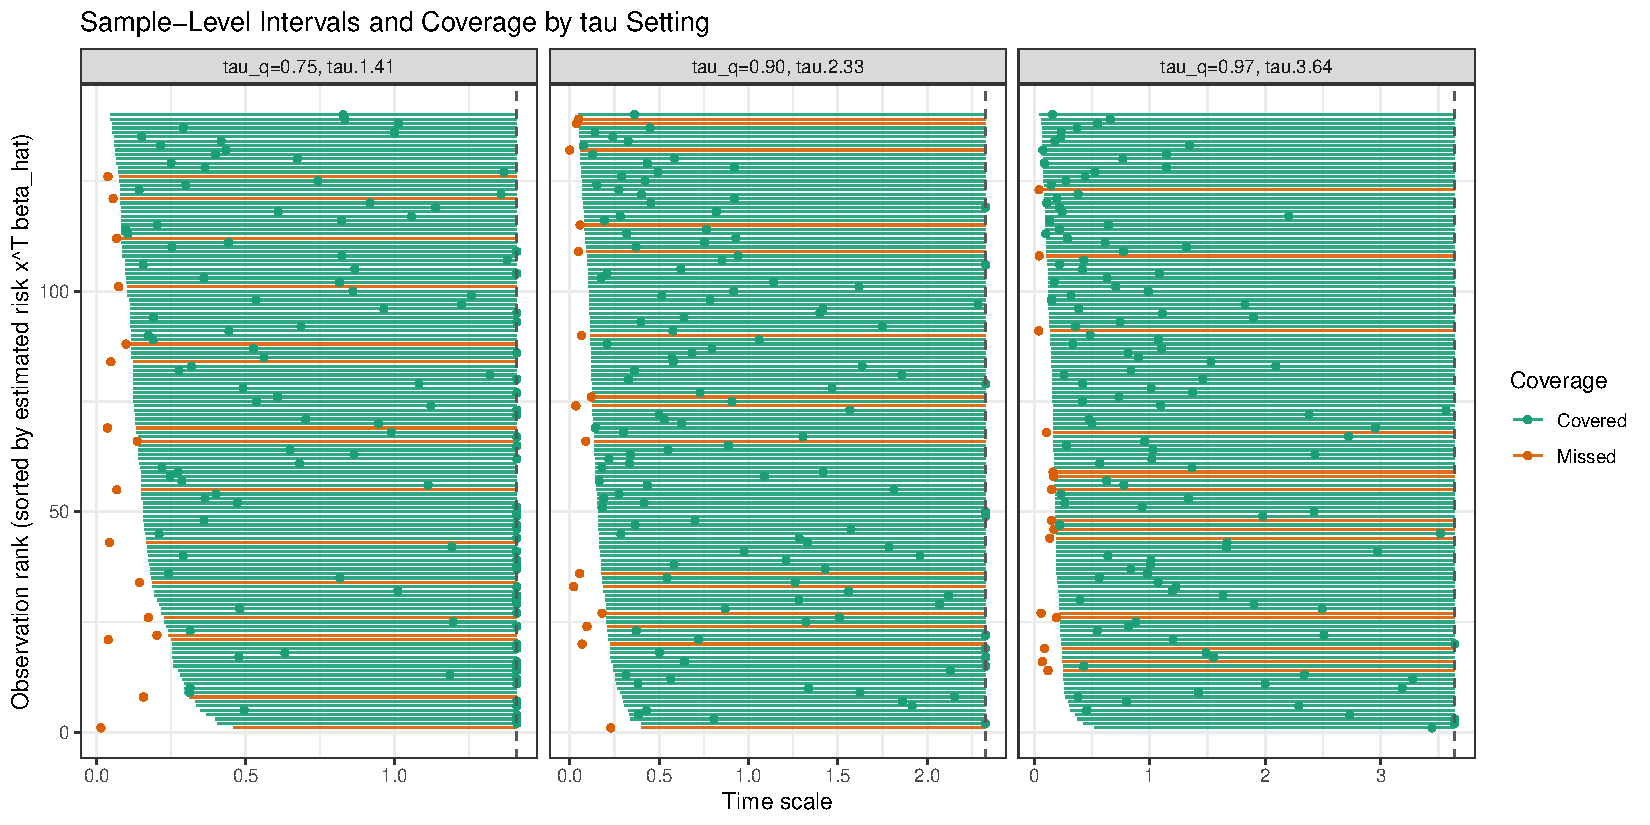
\includegraphics[width=\linewidth]{Figures/direct_interval_coverage_examples.pdf}
  \caption{\textcolor{revisionblue}{Empirical interval coverage examples.}}
  \label{fig:sim_cov_examples}
\end{subfigure}

\vspace{0.7em}
\begin{subfigure}[t]{0.82\textwidth}
  \centering
  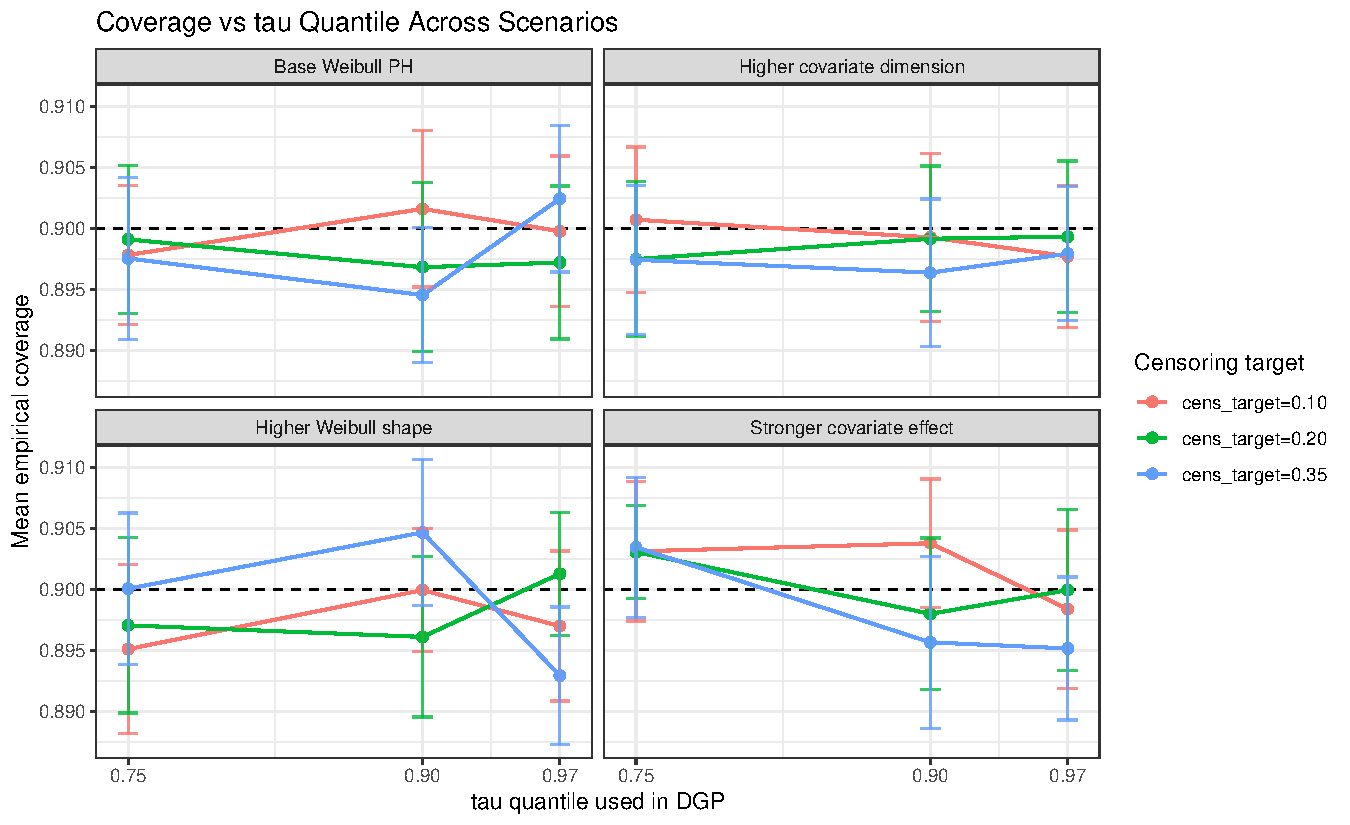
\includegraphics[width=\linewidth]{Figures/coverage_vs_tau.pdf}
  \caption{\textcolor{revisionblue}{Coverage versus $\tau$ quantile.}}
  \label{fig:sim_cov_tau}
\end{subfigure}
\caption{\textcolor{revisionblue}{Simulation results for finite-window conformal predictive intervals under
varying DGP, censoring targets, and $\tau$ settings, with emphasis on empirical
coverage. (a) Direct sample-level intervals and coverage status. (b) Coverage versus
$\tau$ quantile with nominal line and replicate-level uncertainty bars.}}
\label{fig:sim_results_cov}
\end{figure}



\begin{figure}[htbp]
\centering
\begin{subfigure}[t]{0.82\textwidth}
  \centering
  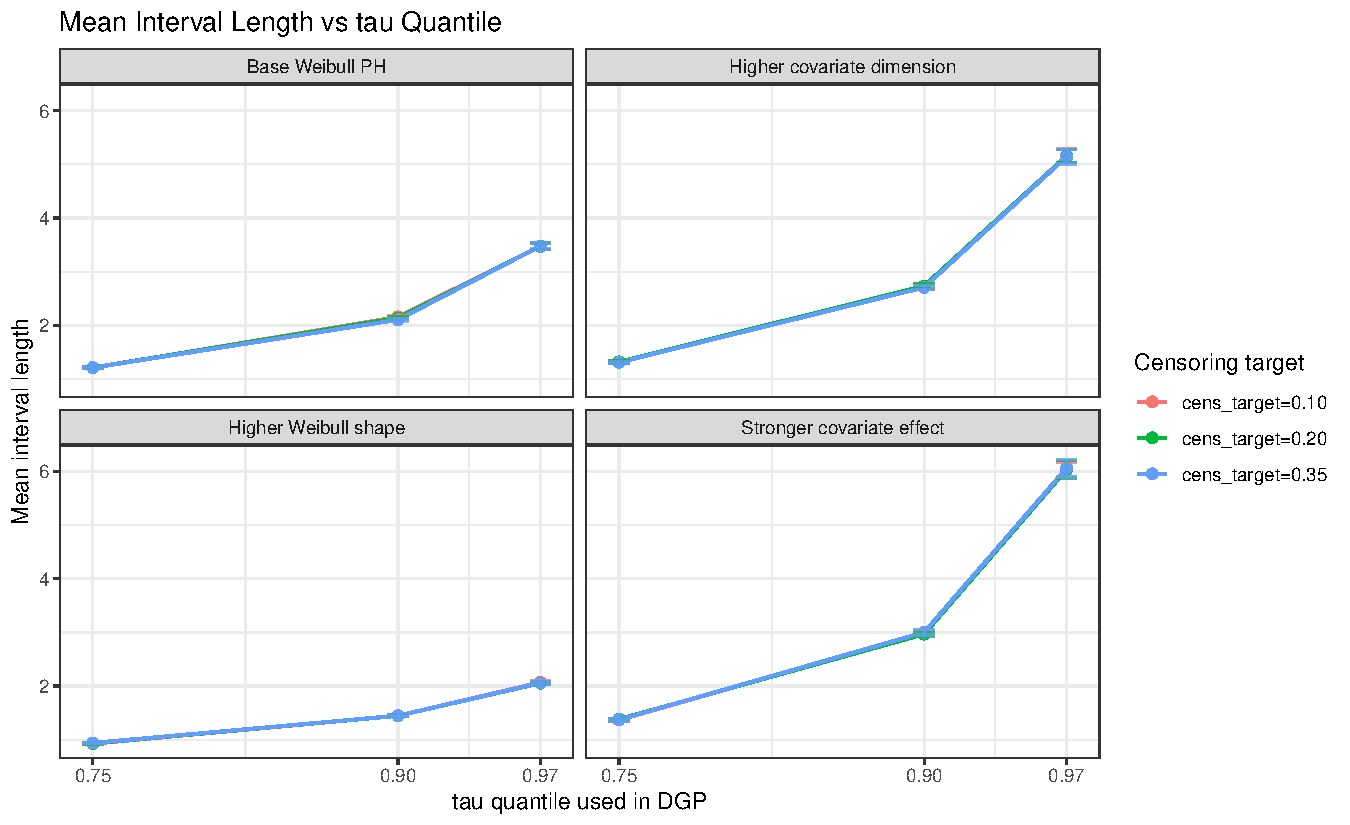
\includegraphics[width=\linewidth]{Figures/length_vs_tau.pdf}
  \caption{\textcolor{revisionblue}{Mean interval length versus $\tau$ quantile.}}
  \label{fig:sim_len_tau}
\end{subfigure}

\vspace{0.7em}
\begin{subfigure}[t]{0.82\textwidth}
  \centering
  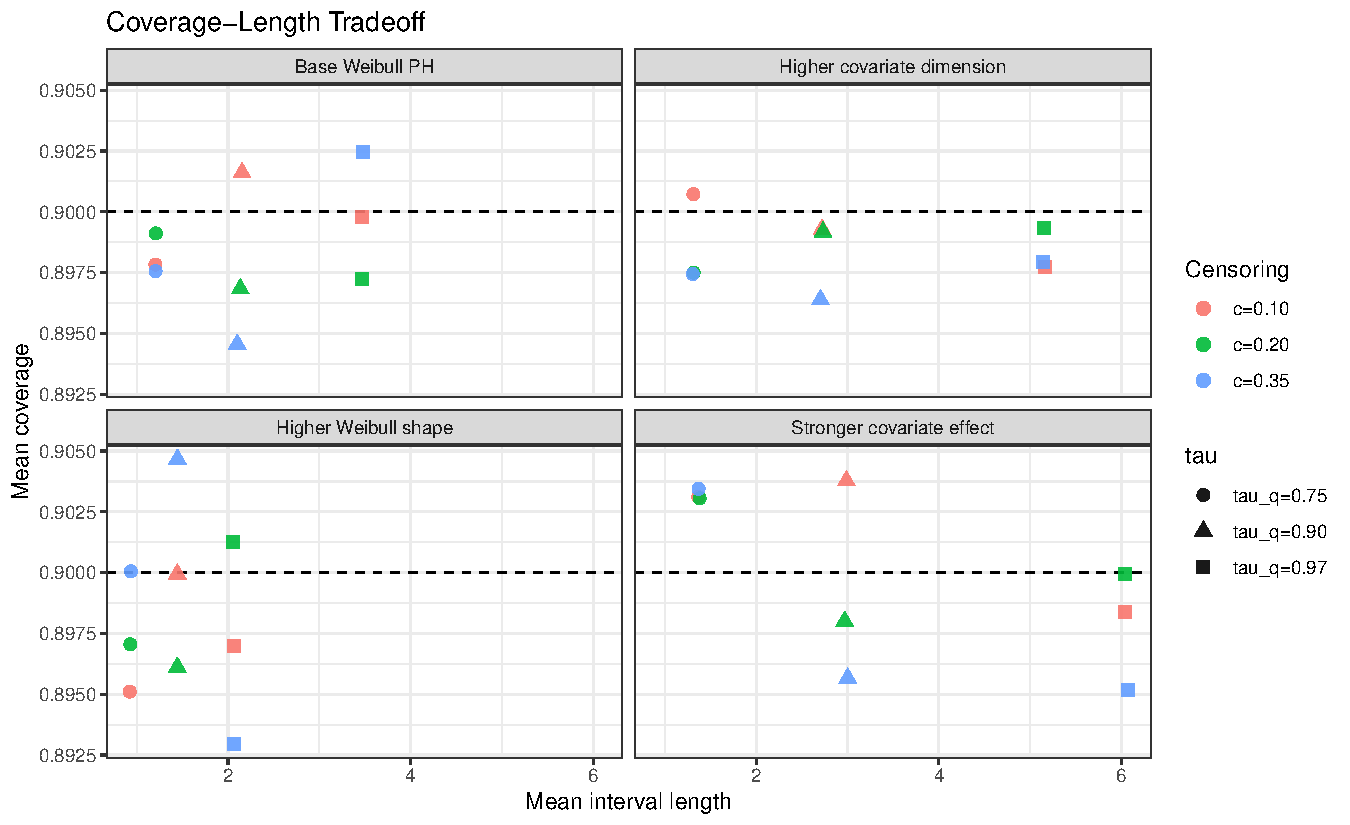
\includegraphics[width=\linewidth]{Figures/coverage_length_tradeoff.pdf}
  \caption{\textcolor{revisionblue}{Coverage-length tradeoff.}}
  \label{fig:sim_len_tradeoff}
\end{subfigure}
\caption{\textcolor{revisionblue}{Simulation results for finite-window conformal predictive intervals under
varying DGP, censoring targets, and $\tau$ settings, with emphasis on interval
length. (a) Mean interval length versus $\tau$ quantile. (b) Coverage-length
tradeoff across settings.}}
\label{fig:sim_results_len}
\end{figure}


{\color{revisionblue}
Across all settings, the overall mean empirical coverage is $0.899$ for target
$0.900$, indicating that the revised upper-$\tau$ conformal construction remains
well calibrated under finite-window truncation.

Figures~\ref{fig:sim_results_cov} and \ref{fig:sim_results_len} present the
simulation results. In Figure~\ref{fig:sim_cov_examples}, each horizontal line
segment is one predicted interval $[\widehat L_i,\tau]$ for a randomly sampled
subset of test observations, ordered by estimated risk score $z^\top\widehat\beta$,
and the dot on that segment is the corresponding true value $T_i^*$. Because the
upper endpoint is fixed at $\tau$, all intervals terminate at the vertical dashed
line marking the realized study horizon in that facet; variation across subjects is
therefore entirely driven by the lower endpoint. Green means covered and orange means
missed. In Figure~\ref{fig:sim_cov_tau}, the $x$-axis is the $\tau$ quantile used in
data generation and the $y$-axis is mean empirical coverage; colors indicate
censoring targets, error bars are 95\% CIs across replicates, and the dashed
horizontal line is nominal coverage $0.9$. Figure~\ref{fig:sim_len_tau} reports the
corresponding mean interval lengths, and Figure~\ref{fig:sim_len_tradeoff}
summarizes the coverage-length tradeoff across settings.

The main qualitative conclusion is that empirical coverage remains very stable across different simulation settings. Averaging over censoring and
$\tau$ settings, mean coverage is $0.899$ in the baseline scenario, $0.900$ under
stronger covariate effects, $0.898$ under higher Weibull shape, and $0.898$ in the
higher-dimensional setting. Averaging over DGP and censoring settings, the mean
coverage is $0.899$, $0.899$, and $0.898$ at $\tau$ quantiles $0.75$, $0.90$, and
$0.97$, respectively, so there is no meaningful drift as administrative truncation
becomes weaker.

Interval length, by contrast, changes substantially with the simulation regime.
Averaged over all DGPs and censoring targets, mean interval length increases from
$1.21$ at $\tau_q=0.75$ to $2.32$ at $\tau_q=0.90$ and $4.18$ at $\tau_q=0.97$,
which is expected because the support of $T^*$ widens as the administrative horizon
moves outward. Averaging over censoring and $\tau$ settings, mean interval length is
$2.27$ in the baseline scenario, $3.47$ under stronger covariate effects, $1.48$
under higher Weibull shape, and $3.06$ in the higher-dimensional setting. Thus the
revised conformal method preserves near-nominal coverage across the full simulation
grid, while efficiency remains sensitive to signal strength, tail behavior, and
covariate dimension.
}

\section{\texorpdfstring{\textcolor{revisionblue}{Expanded Baseline Working-Model Comparison}}{Expanded Baseline Working-Model Comparison}}
\label{sec:expanded_baseline_comparison}
{\color{revisionblue}
We next conduct a full baseline comparison that varies both the working survival model and the degree of administrative truncation. The prediction target remains
\[
T^*=\min(T,\tau).
\]
The goal is to separate three issues that are intertwined in the simple baseline comparison: the effect of correct versus incorrect working models, the role of conformal calibration, and the effect of the finite observation window itself.

\subsection{Methods Compared}
Let $\widehat S_m(t\mid z)$ and $\widehat F_m(t\mid z)=1-\widehat S_m(t\mid z)$ denote the fitted conditional survival and distribution functions under model $m$. Because the target is $T^*$ rather than $T$, the relevant fitted distribution is the mixed finite-window distribution
\[
\widehat F_{m,T^*}(t\mid z)
=
\begin{cases}
\widehat F_m(t\mid z), & 0\le t<\tau,\\
1, & t\ge \tau,
\end{cases}
\qquad
\widehat Q_{m,T^*}(q\mid z)
=
\inf\{t:\widehat F_{m,T^*}(t\mid z)\ge q\}.
\]

For the non-conformal plug-in procedures, for the same reason, we do \emph{not} first construct a symmetric interval for $T$ and then truncate it to $[0,\tau]$. That construction is systematically conservative once the nominal upper endpoint exceeds $\tau$, because the target distribution of $T^*$ has a point mass at $\tau$. Instead, each plug-in comparator fixes the upper endpoint at $\tau$ and assigns the full tail error to the lower side:
\[
\widehat C_m^{\mathrm{plug}}(z)
=
\left[
\widehat Q_{m,T^*}(\alpha\mid z),\;
\tau
\right].
\]
This directly targets the mixed distribution of $T^*$ and removes the structural over-coverage induced by symmetric truncation. This is also consistent in target with the main conformal algorithm with introduced before.

For the conformal procedures, we use the same upper-$\tau$ finite-window algorithm as in the main method, but we now experiment with different working models. For each model $m$, define the working-model pivot
\[
U_m=\widehat S_m(T^*\mid Z).
\]
Let $\widehat c_{m,1-\alpha}$ be the empirical $(1-\alpha)$ quantile of the simulated pivot draws from the estimated finite-window support distribution. The resulting conformal interval is
\[
\widehat C_m^{\mathrm{CP}}(z)
=
\left[
\widehat Q_{m,T^*}(1-\widehat c_{m,1-\alpha}\mid z),\;
\tau
\right].
\]
Under this experiment setting, all six fitted methods return predictive intervals of the common form
$[\text{lower}(z),\tau]$, which makes the comparison directly aligned across
plug-in and conformal procedures.

The six fitted methods are summarized in Table~\ref{tab:expanded_baseline_methods}. The two correctly specified working models under the baseline data-generating process are Weibull and Cox, and the misspecified parametric working model is log-normal.

\begin{table}[htbp]
\centering
\small
\caption{Methods included in the expanded baseline working-model comparison.}
\label{tab:expanded_baseline_methods}
\begin{tabular}{@{}L{0.27\textwidth}L{0.24\textwidth}L{0.41\textwidth}@{}}
\toprule
Method & Working model and interval & Implementation \\
\midrule
Weibull Plug-in & Correctly specified parametric working model with interval $[\widehat Q_{m,T^*}(\alpha\mid z),\tau]$ & Fitted by \texttt{survival::survreg(..., dist = "weibull")}; the fitted Weibull survival curve determines $\widehat F_{m,T^*}$ and $\widehat Q_{m,T^*}$. \\
Cox Plug-in & Correctly specified semi-parametric working model with interval $[\widehat Q_{m,T^*}(\alpha\mid z),\tau]$ & Fitted by \texttt{coxph}; $\widehat S_m(t\mid z)=\exp\{-\widehat H_0(t)\exp(z^\top\widehat\beta)\}$ with Breslow baseline hazard estimate. \\
Log-Normal Plug-in & Misspecified parametric working model with interval $[\widehat Q_{m,T^*}(\alpha\mid z),\tau]$ & Fitted by \texttt{survival::survreg(..., dist = "lognormal")}; this model is not compatible with the Weibull proportional hazards DGP. \\
CP + Weibull & Conformal interval $[\widehat Q_{m,T^*}(1-\widehat c_{m,1-\alpha}\mid z),\tau]$ based on a Weibull working model & Uses the finite-window support estimator, Monte Carlo draws from $\widehat F$, and the global empirical $(1-\alpha)$ quantile of the fitted Weibull pivot $\widehat S_m(T^*\mid Z)$. \\
CP + Cox & Conformal interval $[\widehat Q_{m,T^*}(1-\widehat c_{m,1-\alpha}\mid z),\tau]$ based on a Cox working model & This is the same upper-$\tau$ conformal procedure used in the main method, with the Cox pivot and the global empirical $(1-\alpha)$ pivot cutoff. \\
CP + Log-Normal & Conformal interval $[\widehat Q_{m,T^*}(1-\widehat c_{m,1-\alpha}\mid z),\tau]$ based on a log-normal working model & Uses the same upper-$\tau$ conformal calibration scheme, but replaces the Cox pivot by the fitted log-normal survival curve. \\
\bottomrule
\end{tabular}
\end{table}

\subsection{Simulation Setting and Evaluation Metrics}
The data-generating process is the same as in the main baseline simulation. Event times follow the Weibull proportional hazards model
\[
h(t\mid Z)=\frac{\gamma}{\kappa}\left(\frac{t}{\kappa}\right)^{\gamma-1}\exp(Z^\top\beta),
\]
with $\gamma=1.2$, $\kappa=1$, $p=3$, and $\beta_j=0.30$ for all $j$. Covariates are generated independently from $N(0,1)$. Latent censoring is exponential and calibrated so that non-administrative censoring before $\tau$ is approximately $20\%$.

Relative to the main baseline simulation, the only design factor that changes is the administrative horizon. For each replicate, $\tau$ is set to the empirical $0.70$, $0.80$, $0.90$, or $0.99$ quantile of the generated event times. Each setting uses $n=2000$ observations with a $70\%/30\%$ training--test split, target miscoverage level $\alpha=0.10$, and $B=1500$ Monte Carlo draws for each conformal method. Every $\tau$ regime is repeated $30$ times.

For each replicate and method, empirical coverage and mean interval length are evaluated on the test set:
\[
\widehat{\mathrm{Cov}}
=
\frac{1}{n_{\mathrm{test}}}\sum_{i=1}^{n_{\mathrm{test}}}
I\!\left\{\widehat L_i\le T_i^*\le \widehat U_i\right\},
\qquad
\widehat{\mathrm{Len}}
=
\frac{1}{n_{\mathrm{test}}}\sum_{i=1}^{n_{\mathrm{test}}}
(\widehat U_i-\widehat L_i).
\]
Table~\ref{tab:expanded_baseline_summary} reports the replicate means together with $95\%$ $t$-intervals across the $30$ simulation replicates.

\subsection{Results}
{\small
\setlength{\tabcolsep}{4pt}
\renewcommand{\arraystretch}{0.96}
\begin{table}[htbp]
\centering
\caption[Expanded baseline comparison summary]{Comprehensive summary of coverage and interval length by administrative horizon and method in the expanded baseline comparison.}
\label{tab:expanded_baseline_summary}
\begin{tabular}{@{}cL{0.29\textwidth}cL{0.18\textwidth}cL{0.18\textwidth}@{}}
\toprule
$\tau_q$ & Method & Cov. & Cov. $95\%$ CI & Len. & Len. $95\%$ CI \\
\midrule
0.70 & Weibull Plug-in & 0.903 & [0.897, 0.910] & 1.040 & [1.028, 1.053] \\
0.70 & Cox Plug-in & 0.903 & [0.896, 0.910] & 1.040 & [1.028, 1.053] \\
0.70 & Log-Normal Plug-in & 0.911 & [0.905, 0.917] & 1.049 & [1.037, 1.061] \\
0.70 & CP + Weibull & 0.903 & [0.896, 0.910] & 1.040 & [1.026, 1.054] \\
0.70 & CP + Cox & 0.904 & [0.896, 0.911] & 1.041 & [1.027, 1.055] \\
0.70 & CP + Log-Normal & 0.904 & [0.897, 0.912] & 1.038 & [1.024, 1.053] \\
\midrule
0.80 & Weibull Plug-in & 0.900 & [0.895, 0.905] & 1.424 & [1.408, 1.439] \\
0.80 & Cox Plug-in & 0.901 & [0.895, 0.907] & 1.424 & [1.408, 1.440] \\
0.80 & Log-Normal Plug-in & 0.907 & [0.902, 0.912] & 1.430 & [1.414, 1.446] \\
0.80 & CP + Weibull & 0.900 & [0.893, 0.907] & 1.424 & [1.407, 1.441] \\
0.80 & CP + Cox & 0.903 & [0.896, 0.909] & 1.426 & [1.411, 1.442] \\
0.80 & CP + Log-Normal & 0.901 & [0.894, 0.907] & 1.422 & [1.405, 1.439] \\
\midrule
0.90 & Weibull Plug-in & 0.898 & [0.892, 0.904] & 2.143 & [2.120, 2.165] \\
0.90 & Cox Plug-in & 0.897 & [0.891, 0.902] & 2.142 & [2.120, 2.165] \\
0.90 & Log-Normal Plug-in & 0.903 & [0.896, 0.909] & 2.148 & [2.126, 2.170] \\
0.90 & CP + Weibull & 0.895 & [0.889, 0.901] & 2.139 & [2.116, 2.163] \\
0.90 & CP + Cox & 0.896 & [0.890, 0.902] & 2.140 & [2.118, 2.162] \\
0.90 & CP + Log-Normal & 0.901 & [0.895, 0.907] & 2.143 & [2.120, 2.167] \\
\midrule
0.99 & Weibull Plug-in & 0.897 & [0.891, 0.902] & 4.744 & [4.613, 4.874] \\
0.99 & Cox Plug-in & 0.895 & [0.889, 0.901] & 4.742 & [4.613, 4.872] \\
0.99 & Log-Normal Plug-in & 0.897 & [0.892, 0.903] & 4.745 & [4.614, 4.875] \\
0.99 & CP + Weibull & 0.897 & [0.891, 0.903] & 4.743 & [4.613, 4.872] \\
0.99 & CP + Cox & 0.894 & [0.887, 0.901] & 4.740 & [4.610, 4.871] \\
0.99 & CP + Log-Normal & 0.897 & [0.891, 0.903] & 4.742 & [4.613, 4.871] \\
\bottomrule
\end{tabular}
\end{table}
}

\begin{figure}[htbp]
\centering
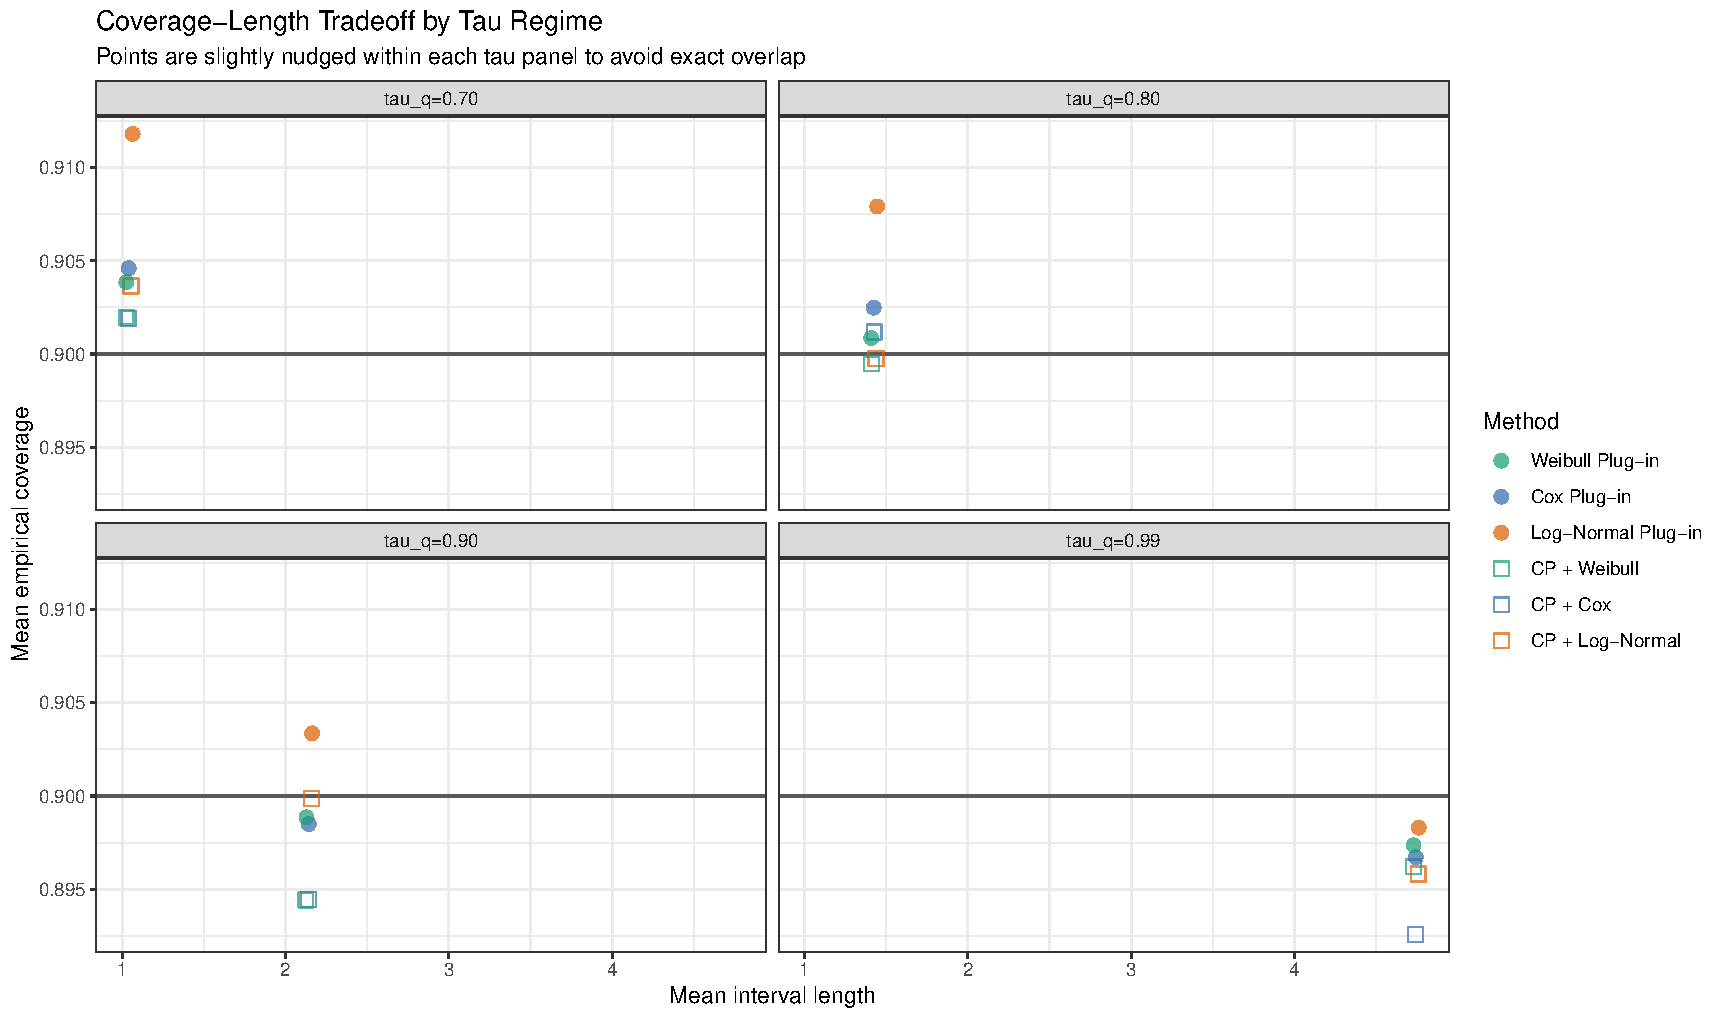
\includegraphics[width=0.92\textwidth]{Figures/model_comparison_uppertau_tradeoff.pdf}
\caption[Coverage--length tradeoff in expanded baseline comparison]{Coverage--length tradeoff by administrative horizon. Each panel corresponds to one $\tau$ regime. After imposing the common upper-$\tau$ interval form, plug-in and conformal procedures with the same working model lie almost on top of one another.}
\label{fig:expanded_baseline_tradeoff}
\end{figure}

Table~\ref{tab:expanded_baseline_summary} together with Figure~\ref{fig:expanded_baseline_tradeoff} show that for correctly specified models (Weibull and Cox), there is essentially no difference between using and not using conformal calibration. For the correctly specified Weibull model, the plug-in and conformal coverages are both $0.903$ at $\tau_q=0.70$, both $0.900$ at $\tau_q=0.80$, and both $0.897$ at $\tau_q=0.99$ up to the third decimal. The same pattern appears for the Cox working model, where the plug-in and conformal coverages differ by at most $0.002$ over the four horizons. 

In contrast, for the misspecified model (Log-normal), the parametric plug-in predictions yield worse coverage, while the conformal calibration procedure maintains near-nominal coverage even though the working model is incorrect. At $\tau_q=0.70$, the log-normal plug-in coverage is $0.911$ and CP + Log-Normal is $0.904$; at $\tau_q=0.80$, the corresponding values are $0.907$ and $0.901$. These differences shrink as $\tau$ increases, and by $\tau_q=0.99$ both methods are essentially aligned at $0.897$ coverage with mean length about $4.74$.

Interval length behaves in a similar way across all six methods. Averaging over the four $\tau$ regimes, mean interval length is $2.338$ for the Weibull plug-in and $2.337$ for CP + Weibull; the corresponding Cox values are both $2.337$. At the widest horizon $\tau_q=0.99$, all four correctly specified procedures have mean lengths essentially equal to $4.74$.

Overall, all six procedures target the same interval form $[\text{lower}(z),\tau]$, and most of them return very accurate coverage. The misspecified log-normal method shows conservativeness at smaller horizons, but this improves when it is paired with the conformal calibration procedure.

As an additional sanity check, we evaluated the correct Weibull plug-in interval using the \emph{true} Weibull DGP parameters instead of estimated parameters. In this oracle calculation, no model fitting is required and the interval remains $[\widehat Q_{T^*}(\alpha\mid z),\tau]$ with the true conditional distribution of $T^*$. The resulting coverage is essentially flat at the nominal level across all horizons, as shown in Table~\ref{tab:expanded_baseline_oracle}. This confirms that the upper-$\tau$ construction itself is correctly targeted; the mild downward drift visible in the fitted Weibull and Cox plug-in curves is a finite-sample estimation effect rather than a structural error of the interval definition.

\begin{table}[htbp]
\centering
\small
\caption{Oracle sanity check for the correctly specified Weibull plug-in interval with upper endpoint fixed at $\tau$.}
\label{tab:expanded_baseline_oracle}
\begin{tabular}{@{}cccc@{}}
\toprule
$\tau_q$ & Oracle coverage & Oracle mean length & Note \\
\midrule
0.70 & 0.900 & 1.031 & True Weibull parameters used \\
0.80 & 0.900 & 1.427 & True Weibull parameters used \\
0.90 & 0.900 & 2.133 & True Weibull parameters used \\
0.99 & 0.900 & 4.829 & True Weibull parameters used \\
\bottomrule
\end{tabular}
\end{table}

\subsection{Harder DGP Robustness Check}
Because the baseline Weibull proportional hazards design is relatively regular and favorable to the Cox working model, we also considered two harder finite-window DGPs as an additional robustness check. The first is a linear log-normal AFT model, under which the log-normal working model is correct while Cox and Weibull are misspecified. The second is a nonlinear log-normal AFT model, under which all three working models are misspecified. This comparison uses the same outer simulation settings as the expanded baseline experiment above: $n=2000$, a $70\%/30\%$ train--test split, $B=1500$, $\tau_q\in\{0.70,0.80,0.90,0.99\}$, and $30$ simulation replicates.

\begin{figure}[htbp]
\centering
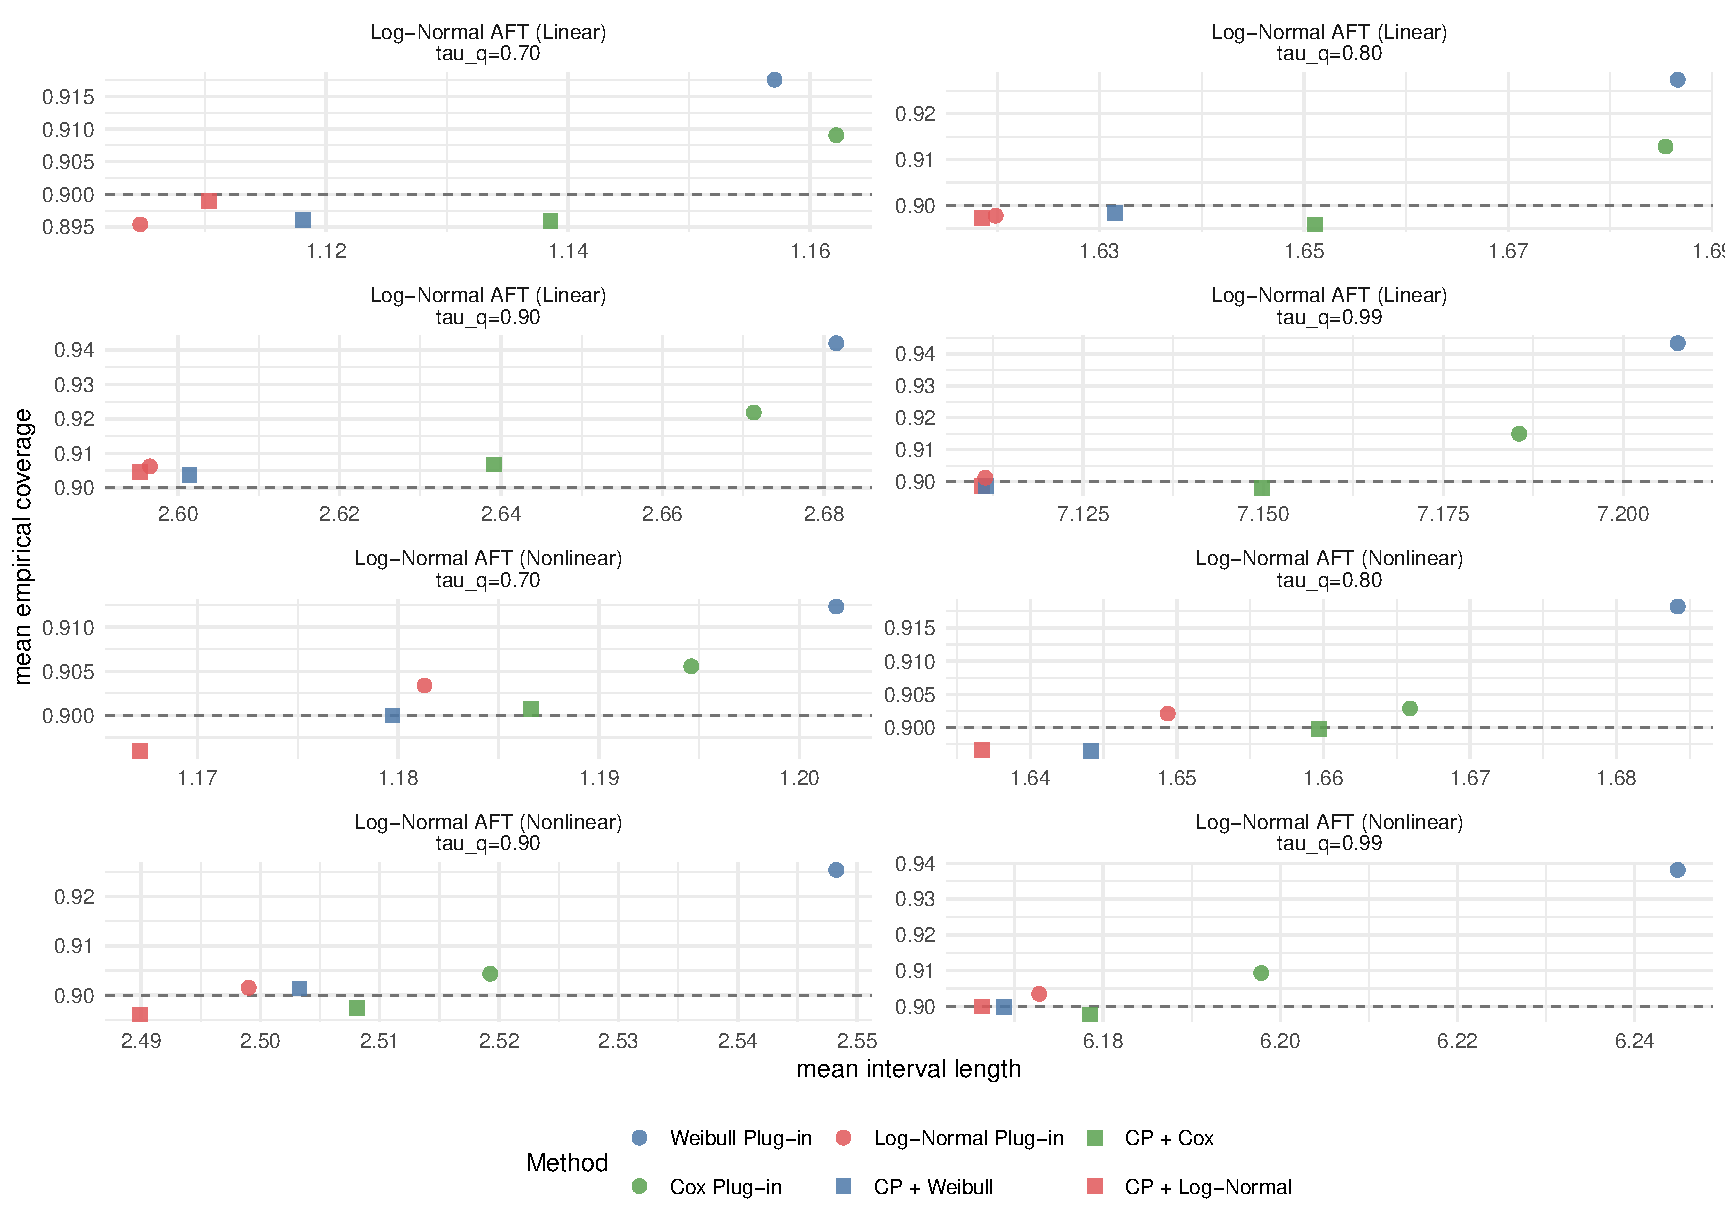
\includegraphics[width=0.96\textwidth]{Figures/challenging_dgp_tradeoff_by_tau.pdf}
\caption[Coverage--length tradeoff under harder DGPs]{Coverage--length tradeoff under two harder finite-window DGPs. The top row corresponds to a linear log-normal AFT model, and the bottom row corresponds to a nonlinear log-normal AFT model.}
\label{fig:challenging_dgp_tradeoff}
\end{figure}

Figure~\ref{fig:challenging_dgp_tradeoff} shows a clearer separation between methods than in the regular baseline setting. Under the linear log-normal AFT DGP, the correctly specified log-normal plug-in method performs well, whereas the misspecified Cox and Weibull plug-in methods are more conservative. Their conformal counterparts move coverage closer to the nominal level and are slightly shorter. Under the nonlinear log-normal AFT DGP, all three working models are misspecified; in this setting, the conformal procedures cluster near nominal coverage, whereas the plug-in methods remain mildly conservative, with the Weibull plug-in showing the largest deviation. Overall, this harder-DGP check supports the same qualitative conclusion as before: conformal calibration is most useful when the working model is incorrect, while the direct plug-in approach can still perform well when the model is correctly specified. Another notable pattern is that when the linear log-normal AFT model is correct, CP + Log-Normal achieves the best efficiency among the CP-based methods and is essentially as efficient as the correctly specified parametric method. When all parametric and CP-based working models are misspecified, CP combined with the more nearly correct log-normal working model again gives the best efficiency among the competing methods. This suggests that conformal calibration can provide additional benefit when it is paired with a working model that captures more of the underlying data-generating mechanism.
}

\section{\texorpdfstring{\textcolor{revisionblue}{Split-Sample Sensitivity Check}}{Split-Sample Sensitivity Check}}
{\color{revisionblue}
The main conformal algorithm uses the same training sample both to estimate the weighted finite-window support distribution of $(T^*,Z)$ and to fit the Cox working model. As a sensitivity check, we also considered a half-split variant in which the sample is divided into two equal parts: one half is used only for support estimation, while the other half is used only to fit the Cox working model, to reduce the dependence between training and calibration. This experiment uses the same outer settings as the harder-DGP check above: $n=2000$, a $70\%/30\%$ training--test split, $B=1500$ Monte Carlo draws, $\tau_q\in\{0.70,0.80,0.90,0.99\}$, and $30$ replicates for each of the two harder DGPs.

\begin{table}[htbp]
\centering
\small
\caption{\textcolor{revisionblue}{Average coverage and mean interval length for the original CP + Cox method and the half-split variant, aggregated over $\tau$ within each harder DGP.}}
\label{tab:splitcheck_summary}
\resizebox{0.95\textwidth}{!}{%
\begin{tabular}{@{}ccccc@{}}
\toprule
Scenario & CP + Cox Cov. & Half-Split Cov. & CP + Cox Len. & Half-Split Len. \\
\midrule
Linear log-normal AFT & 0.897 & 0.898 & 3.167 & 3.167 \\
Nonlinear log-normal AFT & 0.899 & 0.901 & 2.907 & 2.909 \\
\bottomrule
\end{tabular}
}%
\end{table}

Table~\ref{tab:splitcheck_summary} shows that under the harder DGPs, the half-split variant behaves almost identically to the original CP + Cox procedure. In the linear log-normal AFT setting, coverage changes from $0.897$ to $0.898$ with essentially no change in mean interval length; in the nonlinear setting, coverage changes from $0.899$ to $0.901$, again with virtually no change in length. This suggests that separating support estimation from working-model fitting does not materially change the empirical behavior of the method in these experiments.
}



\chapter{Discussion}
This thesis develops and studies conformal predictive intervals for right-censored survival outcomes when the practical inferential target is the finite-window quantity $T^*=\min(T,\tau)$.
The methodology integrates IPCW-based estimation of the joint distribution of $(T^*,Z)$ with a Cox-based pivot and Monte Carlo conformal calibration.

From simulation experiments, three main empirical findings emerge.
First, the finite-window conformal interval maintains near-nominal marginal coverage across a broad range of censoring and data-generating settings.
Second, interval width responds predictably to the horizon parameter $\tau$ and scenario difficulty.
Third, in the expanded baseline working-model comparison and the harder-DGP check, correctly specified parametric models perform well across settings. Conformal procedures, whether paired with a correct or incorrect working model, achieve coverage and efficiency comparable to those of the correctly specified parametric methods, with more accurate working models tending to be the most efficient among the CP-based procedures. Incorrect parametric models perform worse, as expected. Taken together, these comparisons support the robustness and efficiency of the proposed conformal method for predicting time to event under finite follow-up.

From a more practical perspective, the proposed method can address several clinically relevant questions in a fixed-horizon study. For an individual patient, it provides a plausible time range for the event to occur within the finite follow-up window at a prespecified confidence level. Equivalently, the lower endpoint gives a confidence-calibrated statement about how long the patient is expected to remain event-free. It can also address milestone-based questions, such as how confidently we can say that a patient will remain event-free beyond a clinically important time point (e.g.\ 1, 3, or 5 years). Finally, because the method produces lower predictive bounds for all patients, it can help identify individuals with shorter predicted event-free time who may require closer monitoring or earlier intervention.

Several limitations remain. First, the method uses a recovered joint distribution to generate synthetic calibration samples. This avoids more complicated weighting and adjustment within the conformal procedure, but it also introduces reliance on the quality of $\hat F$ estimation, and finite-sample exchangeability in the original conformal sense is not guaranteed. Second, the harder-DGP results reveal some interesting patterns in how the correctness of the working model affects predictive efficiency, but these patterns have not yet been explored theoretically. Finally, the current study is limited to simulation and still lacks solid real-world data applications. 

Ongoing work and future directions include (1) theoretical explorations of the underlying relationship between correctness of working models and efficiency of conformal predictive intervals in survival analysis. (2) methodological extension to more practical and complicated survival scenarios including competing risk data and categorical cause type predictions. (3) application to large-scale real-world datasets like the ADNI (Alzheimer’s Disease Neuroimaging Initiative) database.


\clearpage
\addchaptertoc{References}
\bibliography{Citations}

\normalsize
\nonfrenchspacing
\doublespacing
\setlength{\parindent}{15pt}
\setlength{\parskip}{3pt}

\end{document}
